% Homework template for Algorithm Analysis and Design
% UPDATE: September 20, 2019 by Xu Rongchen
\documentclass[a4paper]{article}
\usepackage{ctex}
\ctexset{
proofname = \heiti{证明} %% set proof name
}
\usepackage{amsmath, amssymb, amsthm}
% amsmath: equation*, amssymb: mathbb, amsthm: proof
\usepackage{moreenum}
\usepackage{mathtools}
\usepackage{url}
\usepackage{bm}
\usepackage{enumitem}
\usepackage{graphicx}
\usepackage{subcaption}
\usepackage{booktabs} % toprule
\usepackage[mathcal]{eucal}

\usepackage{iidef} % set homework count
\usepackage{longtable}

% \usepackage[noend]{algpseudocode}
\usepackage{clrscode3e}

\thecoursename{算法分析与设计实验报告}
\theterm{2019年秋季学期}
\hwname{排序算法比较}
\slname{\heiti{解}}
\begin{document}
\courseheader
\theusername{徐荣琛}
\thestuno{2019214518}
\theinstitute{软件学院}

\info

\begin{enumerate}
  \setlength{\itemsep}{3\parskip}
  %% Homework Start here:
  %% \item to enumerate the problem ID: Format as 'HomeworkID.ProblemID'
  %% \begin{solution} XXXX \end{solution} is to make a solution
  %% \begin{proof} XXXX \end{proof} is to make a proof
  %% Suggest to use \input{path} command
  \textbf{1.实验要求}\\
  比较insertionsort,shellsort,quicksort,mergesort以及radixsort对32位无
  符号整数的排序效果,要求给出一个实验报告。输入数据随机产生,数据范围为[0,$2^{32}-1$],
  输入数据量分别为:$10$,$10^2$,$10^3$,$10^4$,$10^5$,$10^6$,$10^7$,$10^8$,
  $2\times10^8$,($10^9$,此数量级选做)。\\
  \bigskip

  \textbf{2.实验环境}\\
  为了提高代码运行效率,此次实验代码采用C++语言实现,具体的实验环境及编译配置如下表所示:\\ \medskip
  \begin{tabular}{c|c}
    \hline\hline
    处理器 & Intel(R) Core(TM) i7-8850H CPU @ 2.60GHz \\ \hline
    内存 & 16GB\\ \hline
    操作系统& Mac OS X 10.14.6\\ \hline
    CMake版本& 3.14.1\\ \hline
    编译器& clang 11.0.0(C++14)\\ \hline
    Release编译参数& -O3\\
    \hline\hline
  \end{tabular}\\
  \bigskip

  \textbf{3.实验内容}\\
  \textbf{3.1 有关算法的实现}\\
  \medskip
  3.1.1 Insertion Sort:\\
  从数组第二个元素开始,逐一和前项比较,如果比前项小,则继续向前比较,否则停止这个元素的
  比较,并进入下一元素;\\
  \medskip
  3.1.2 Shell Sort:\\
  Shell Sort采用一个递减间隔序列$D$(最终为1),对于$D$中每一项$d_i$,对数组中每个距离
  $d_i$的子序列进行Insertion Sort。由于最终的间隔为1,保证了最后结果一定有序;\\
  \medskip
  3.1.3 Quick Sort:\\
  Quick Sort采用分治策略,先从数组中选择一个数作为划分依据,随后将所有数按和划分依据的大小关系
  进行分离,保证比划分依据小的数均在划分依据前,大的均在划分依据之后,随后对前后两部分继续递归;\\
  \medskip
  3.1.4 Merge Sort:\\
  Merge Sort亦采用分治策略,首先将数组分为等长的两部分(或长度差为1),对两部部分递归排序,直至
  仅剩一个元素,随后可在线性时间内对有序的两部分进行合并。合并时需要使用$O(n)$的辅助空间;\\
  \medskip
  3.1.5 Radix Sort:\\
  Radix Sort的基数为$R$的情况下,将待排序数表示为$R$进制:$a_0R^0+a_1R^1+a_2R^2+\cdots$,则
  依次对$a_0,a_1,a_2,\cdots$进行Counting Sort。Counting Sort需要使用$O(n)$的辅助空间;\\
  \medskip
  3.1.6 32位随机数生成:\\
  某些平台和C++标准下不能直接生成32位数,可随机出两个16位数,将一个左移16位异或上第二个即可。\\
  \medskip
  \textbf{3.2 部分排序算法的优化}\\
  \medskip
  3.2.1 Shell Sort:\\
  Shell Sort采用的间隔序列最初是采用$n/2,n/4,\cdots$,后经过相关资料查询,发现一个能够表现更优的序列:
  $a(n) = 9*2^n - 9*2^{n/2} + 1$($n$是偶数),$a(n) = 8*2^n - 6*2^{(n+1)/2} + 1$($n$是奇数)。
  实验结果表明,在处理$10^8$数量级的排序数时,原先方法的耗时在26秒左右,优化方法的耗时在16秒左右,
  性能提升比例约38.5\%。\\
  \medskip
  3.2.2 Radix Sort:\\
  考虑到计算机实际结构,基数采用2的幂时应当具备更加的性能。在此基础上,对于一个数获取其对应的Count数组
  下标的方式采用二进制位运算,先将数右移需要的位数,再与上对于的二进制掩码$2^r-1$,即可获得数组下标。
  对于基数的大小,经过反复实验,发现在一定数据规模之上,$r=8$时有最佳的性能表现。\\
  % 3.2.2 Radix Sort:\\
  % Radix Sort采用链表存储作为桶的数据结构,但是实际运行速度较慢,分析其原因可能有两部分组成:\\
  % (1)链式存储的方式使得访存不连续,可能使得每次访问均需要请求内存,而不能从Cache中获得;\\
  % (2)简单的链式存储,每将一个32位数据串联均需要一个额外的64位地址空间,使得需要的初始化内存
  % 较实际扩大3倍,在内存申请和释放时效率降低(同时,同样大小下,非连续空间的内存申请和释放也较
  % 连续空间效率低)。\\
  % 于是优化了桶的数据结构,从简单的链表改为使用块状链表,初始化块大小为$1.01\times\frac{n}{m}$,
  % 增量块大小为$\max(\sqrt{\frac{n}{m}},1)$,其中$n$是数的个数,$m$是桶数。在随机分布的情况下,
  % 初始化块大小保证大多数块不需要再额外附加空间,增量块大小又保证了每次附加空间不显著增加空间消耗。
  % 同时\\
  \medskip
  \textbf{3.3 不同规模下的求解实验}\\
  \medskip
  3.3.1 实验概要:\\
  在$10$,$10^2$,$10^3$,$10^4$,$10^5$,$10^6$,$10^7$,$10^8$,$2\times10^8$
  以及$10^9$的数据规模下对insertionsort,shellsort,quicksort,mergesort和radixsort就行
  性能对比实验,数据按3.1.6的方法生成。为了反应实现性能,增加一组对比组,对比组采用C++标准库中的
  std::sort,它是一种以quicksort为主体的混合策略比较排序算法,具有优异的性能表现。设置每组的超时时间为600秒。实验程
  序编译时设定为Release,采用O3编译优化。\\
  \medskip
  3.4.2 实验结果:\\
  实验结果如下表所示,实验进行三次,表中值为三次的均值,单位为秒。
  \resizebox{\linewidth}{!}{ 
  \begin{tabular}{c||cccccc}
    \hline\hline
    规模          &Insertion  &Shell      &Quick      &Merge      &Radix      &std::sort\\\hline
    $10$          &0.000002   &0.000007   &0.000010   &0.000042   &0.000043   &0.000004 \\
    $10^2$        &0.000009   &0.000013   &0.000012   &0.000032   &0.000037   &0.000009 \\
    $10^3$        &0.000288   &0.000126   &0.000136   &0.000163   &0.000054   &0.000105 \\
    $10^4$        &0.011835   &0.001344   &0.001254   &0.001312   &0.000252   &0.000810 \\
    $10^5$        &0.963522   &0.013011   &0.009247   &0.011309   &0.001479   &0.007179 \\
    $10^6$        &96.303069  &0.118858   &0.074969   &0.094963   &0.013092   &0.063501 \\
    $10^7$        &Timeout    &1.296577   &0.720626   &0.933322   &0.123105   &0.647785 \\
    $10^8$        &Timeout    &15.475431  &7.902971   &10.544991  &1.281067   &7.394379 \\
    $2\times10^8$ &Timeout    &32.764344  &16.328107  &21.922669  &2.338945   &15.293089 \\
    $10^9$        &Timeout    &187.990393 &88.534788  &121.997050 &22.943960  &85.843276 \\
    \hline\hline
  \end{tabular}
  }\\
  \medskip
  3.4.3 实验分析:\\
  以数据规模为横坐标,算法耗时为纵坐标(为方便低数量级的展示,故这里两者均采用对数坐标),绘制出如下的
  耗时曲线比较图:
  \begin{center}
    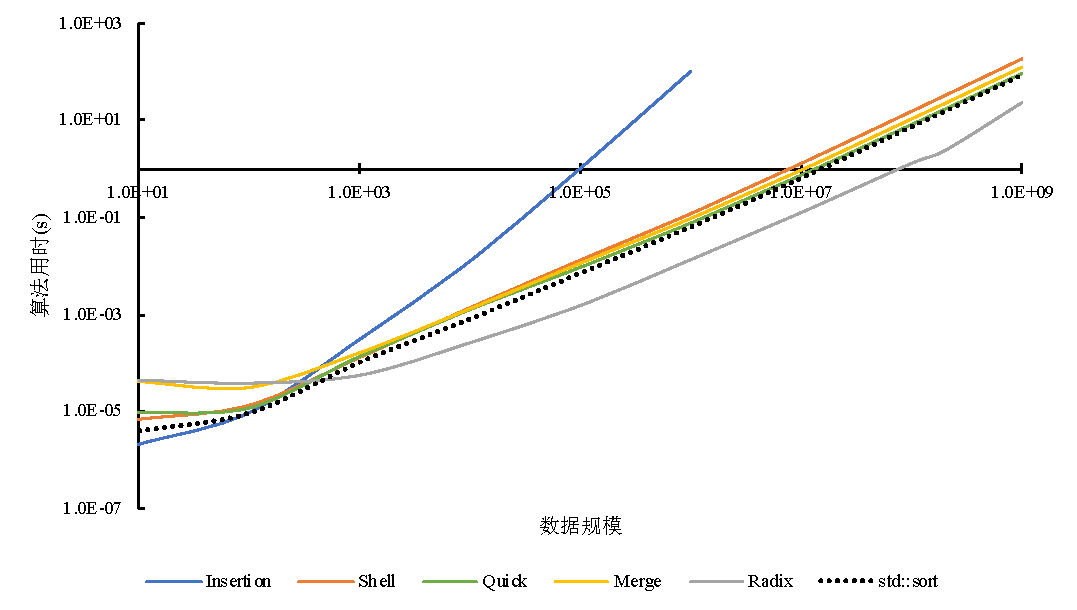
\includegraphics[scale=0.56]{Pictures/SR.pdf}
  \end{center}
  由于部分算法耗时比较接近,为了方便展示,以std::sort为基准,计算其他算法和其的耗时比,绘制出以下的耗时
  比例的曲线图:
  \begin{center}
    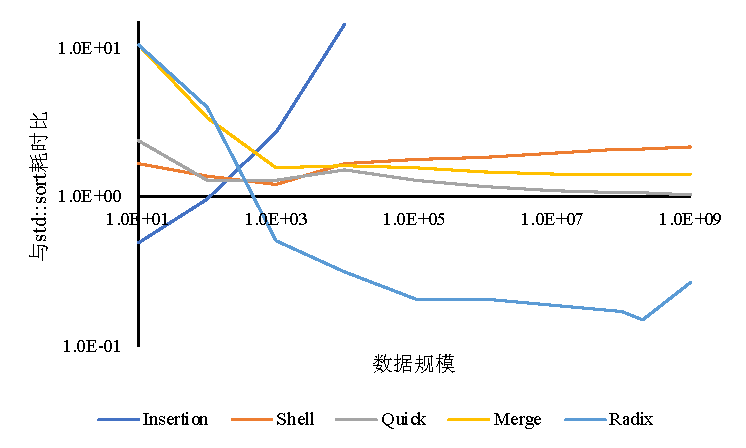
\includegraphics[scale=0.8]{Pictures/SRR.pdf}
  \end{center}
  从图中可发现,当数据规模小于$10^2$数量级时,Insertion排序具有最快的时间效率,但是随之数据规模增加,
  Insertion排序效率迅速恶化。当数据规模大于$10^3$数量级时,Radix排序展现出来了明显的性能优势,甚至
  大幅度领先于std::sort。三个平均复杂度$O(n\lg n)$的比较排序算法中,数据规模较小时Merge排序速度较慢
  但随着规模增大,Merge排序逐渐优于Shell排序,但是仍然劣于Quick排序。Quick排序性能非常接近std::sort,
  这也与预期一致。\\
  值得注意的时Radix排序在$10^9$数据规模时,有一个较为明显的性能恶化。分析其原因,$10^9$的32位数据空间
  为4GB,另外为了保持对比实验有效性,保存了一份同样数据的备份。再加上Radix排序时需要的辅助数组空间,
  内存峰值消耗超过12GB,如果再考虑操作系统以及其它应用程序的内存占用,极有可能整体内存占用超过计算机内存总量
  而发生了一定规模的虚拟内存交换,所以导致了性能下降幅度比较明显。
\end{enumerate}


\end{document}